\documentclass[varwidth]{standalone} % varwidth because of https://tex.stackexchange.com/a/622526/828
\usepackage{subcaption}	% for concatenating images
\usepackage{tikz}				% for drawing everything
\usepackage{siunitx}			% for nice SI units
\newcommand{\imsize}{\linewidth}	% default width of image
\newlength\imagewidth		% needed for correct scalebar
\newlength\imagescale		% needed for correct scalebar
\pgfmathsetlength{\imagewidth}{\imsize}%
\begin{document}
\pagecolor{black}% all black page, to discard the differently sized images
\begin{figure}%
	\begin{subfigure}[c]{0.5\linewidth}%
		\pgfmathsetlength{\imagewidth}{\imsize}%
		\pgfmathsetlength{\imagescale}{\imagewidth/609}%
		\def\x{37.6}% scalebar-x starting at golden ratio of image width of 609px = 376
		\def\y{456}% scalebar-y at 90% of image height of 480px = 432
		\begin{tikzpicture}[x=\imagescale,y=-\imagescale]%
			\node[anchor=north west, inner sep=0pt, outer sep=0pt] at (0,0) {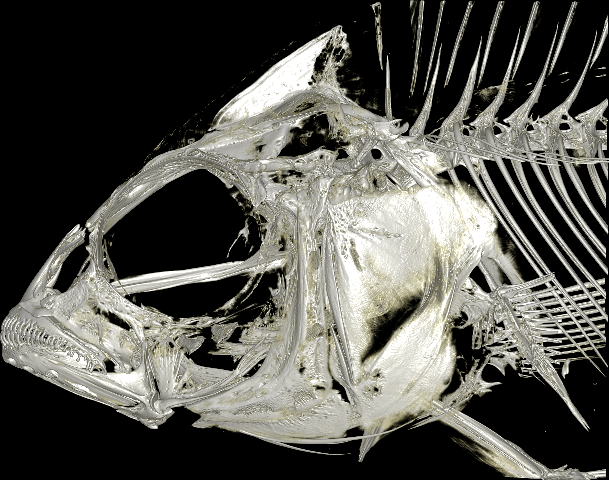
\includegraphics[width=\imagewidth]{104016/head}};
			% 475.587px = 18.486mm -> 100px = 3886.984um -> 12.863px = 500um, 2.573px = 100um
			%\draw[|-|,blue] (5,362) -- (340,25) node [sloped,midway,above,fill=white,semitransparent,text opacity=1] {\SI{18.486}{\milli\meter} (476px)};
			\draw[|-|,white] (\x,\y) -- (\x+128.63,\y) node [right] {\SI{5}{\milli\meter}};
			\draw[color=black, anchor=north west] (0,0) node [fill=white, semitransparent] {A} node {A};
		\end{tikzpicture}%
	\end{subfigure}%
	\begin{subfigure}[c]{.5\linewidth}%
		\pgfmathsetlength{\imagewidth}{\imsize}%
		\pgfmathsetlength{\imagescale}{\imagewidth/1153}%
		\def\x{547}% scalebar-x measured at the center between the two lower jaws
		\def\y{774.25}% scalebar-y at 90% of image height of 815px = 734
		\begin{tikzpicture}[x=\imagescale,y=-\imagescale]
			\node[anchor=north west, inner sep=0pt, outer sep=0pt] at (0,0) {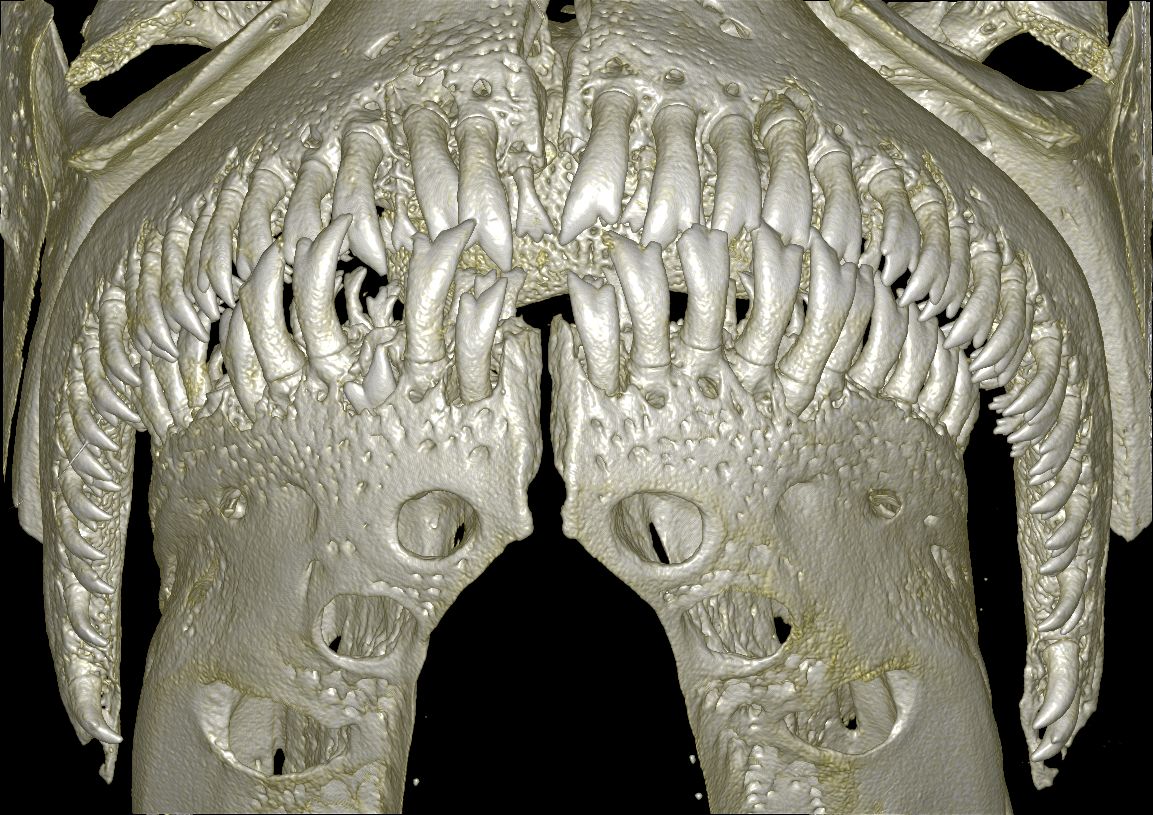
\includegraphics[width=\imagewidth]{104016/oj}};
			% 834.069px = 3.24mm -> 100px = 388.457um -> 128.714px = 500um, 25.743px = 100um
			%\draw[|-|,blue] (144,627) -- (978,594) node [sloped,midway,above,fill=white,semitransparent,text opacity=1] {\SI{3.24}{\milli\meter} (834px)};
			\draw[|-|,white] (\x-128.714/2,\y) -- (\x+128.714/2,\y) node [midway,below] {\SI{500}{\micro\meter}};
			\draw[color=black, anchor=north west] (0,0) node [fill=white, semitransparent] {B} node {B};
		\end{tikzpicture}
	\end{subfigure}\\%
	\begin{subfigure}[c]{.33\linewidth}
		\pgfmathsetlength{\imagewidth}{\imsize}%
		\pgfmathsetlength{\imagescale}{\imagewidth/1124}%
		\def\x{695}% scalebar-x starting at golden ratio of image width of 1124px = 695
		\def\y{551}% scalebar-y at 90% of image height of 580px = 522
		\begin{tikzpicture}[x=\imagescale,y=-\imagescale]
			\node[anchor=north west, inner sep=0pt, outer sep=0pt] at (0,0) {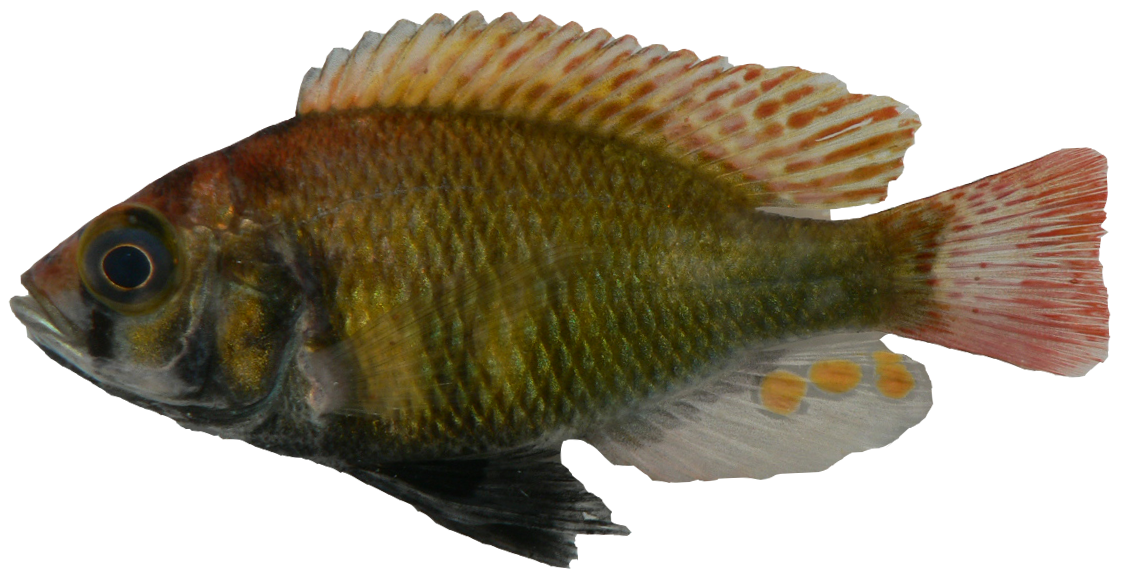
\includegraphics[width=\imagewidth]{104016/fish}};
			% 1090.775px = 70.0mm -> 100px = 6417.455um -> 7.791px = 500um, 1.558px = 100um
			%\draw[|-|,blue] (14,298) -- (1105,281) node [sloped,midway,above,fill=white,semitransparent,text opacity=1] {\SI{70.0}{\milli\meter} (1091px)};
			\draw[|-|,white] (\x,\y) -- (\x+77.91+77.91,\y) node [right] {\SI{1}{\centi\meter}};
			\draw[color=black, anchor=north west] (0,0) node [fill=white, semitransparent] {C} node {C};
		\end{tikzpicture}%
	\end{subfigure}%
	\begin{subfigure}[c]{.33\linewidth}
		\pgfmathsetlength{\imagewidth}{\imsize}%
		\pgfmathsetlength{\imagescale}{\imagewidth/710}%
		\def\x{439}% scalebar-x starting at golden ratio of image width of 710px = 439
		\def\y{664.05}% scalebar-y at 90% of image height of 699px = 629
		\begin{tikzpicture}[x=\imagescale,y=-\imagescale]
			\node[anchor=north west, inner sep=0pt, outer sep=0pt] at (0,0) {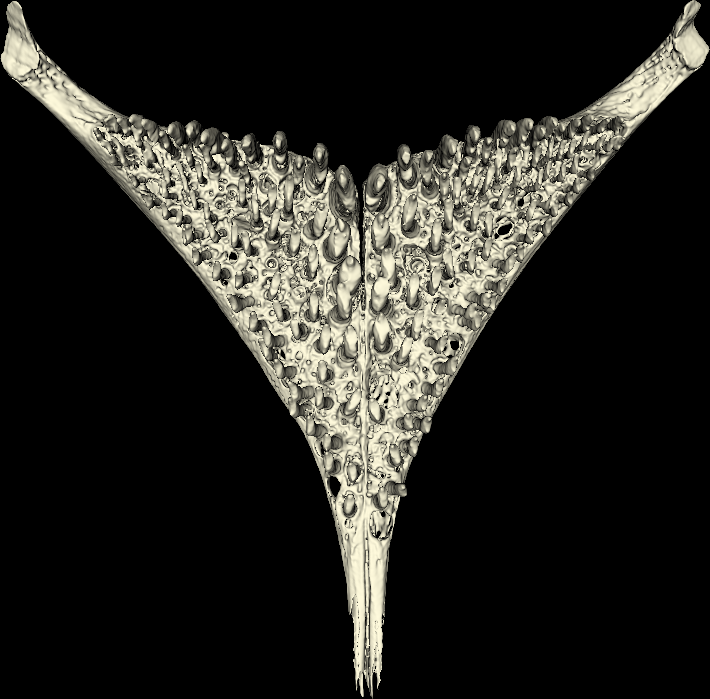
\includegraphics[width=\imagewidth]{104016/pj_top}};
			% 762.062px = 5.475mm -> 100px = 718.446um -> 69.595px = 500um, 13.919px = 100um
			%\draw[|-|,blue] (692,8) -- (362,696) node [sloped,midway,above,fill=white,semitransparent,text opacity=1] {\SI{5.475}{\milli\meter} (762px)};
			\draw[|-|,white] (\x,\y) -- (\x+69.595+69.595,\y) node [right] {\SI{1}{\milli\meter}};
			\draw[color=black, anchor=north west] (0,0) node [fill=white, semitransparent] {D} node {D};
		\end{tikzpicture}%
	\end{subfigure}%
	\begin{subfigure}[c]{.33\linewidth}
		\pgfmathsetlength{\imagewidth}{\imsize}%
		\pgfmathsetlength{\imagescale}{\imagewidth/1112}%
		\def\x{687+100+100}% scalebar-x starting at golden ratio of image width of 1112px = 687
		\def\y{337}% scalebar-y at 90% of image height of 374px = 337
		\begin{tikzpicture}[x=\imagescale,y=-\imagescale]
			\node[anchor=north west, inner sep=0pt, outer sep=0pt] at (0,0) {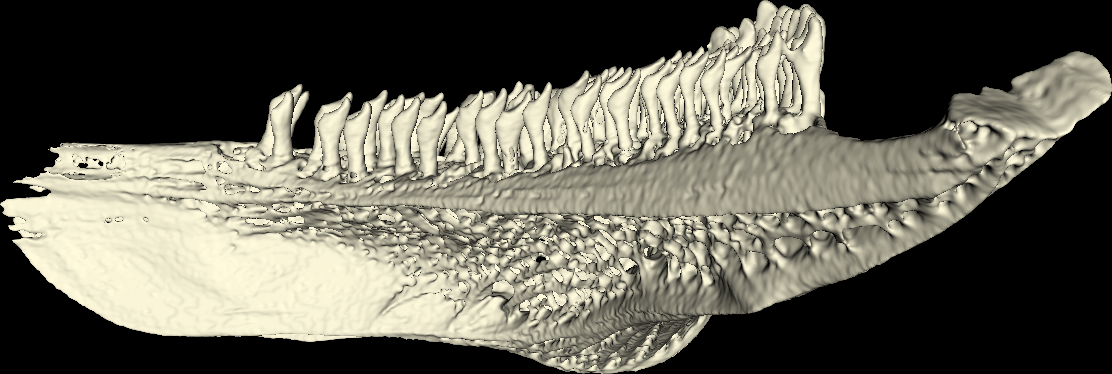
\includegraphics[width=\imagewidth]{104016/pj_side}};
			% 1067.600px = 5.195mm -> 100px = 486.606um -> 102.753px = 500um, 20.551px = 100um
			%\draw[|-|,blue] (46,191) -- (1109,87) node [sloped,midway,above,fill=white,semitransparent,text opacity=1] {\SI{5.195}{\milli\meter} (1068px)};
			\draw[|-|,white] (\x,\y) -- (\x+102.753+102.753/2,\y) node [midway,below] {\SI{750}{\micro\meter}};
			\draw[color=black, anchor=north west] (0,0) node [fill=white, semitransparent] {E} node {E};
		\end{tikzpicture}%
	\end{subfigure}%
\end{figure}
%----------
\end{document}%
